A measurement of the cross section times branching fration of \ttH~(\Hgg)~production is performed by defining regions of the data which are highly enriched in \ttH~events. These regions, called ``signal regions'', are constructed through a set of requirements placed on all candidate events. 
The requirements consist of two components: 
(1) a ``loose preselection'', which selects events with at least some of the expected decay products of the \ttH~system and 
(2) a selection based on the output of a binary classification algorithm (called ``BDT-bkg''), trained to separate \ttH~from the SM background processes. The loose preselection aims to maintain a very high signal efficiency (FIXME: CITE) and provides the phase space in which BDT-bkg is trained.
The BDT-bkg algorithm is trained on MC simulation of signal and background, as well as a data-driven description of some backgrounds. After training the BDT-bkg algorithm, signal regions are constructed by placing requirements on the output of BDT-bkg (on top of the preselection requirements).
Within these signal regions, signal and background models are constructed and a measurement of the \ttH~cross section is calculated by performing a simultaneous fit to events in all of the signal regions. 
%Although the loose preselection maintains an efficiency of X\% (FIXME) on \ttH~events, the SM background is still far too large to perform a precise measurement of the \ttH~cross section. The output of BDT-bkg is then used to construct signal regions.
%
\subsection{The \Hgg~Decay Mode}
The analysis targets \ttH~events in which the Higgs boson decays into two photons (\Hgg). As the photon is a massless particle, it does not couple directly to the Higgs boson.
Instead, the dominant process through which the Higgs boson decays to two photons involves a top quark loop, as shown in Figure~\ref{fig:hgg_feynman}.
\begin{figure}[h!]
    \centering
    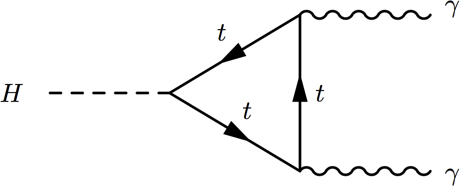
\includegraphics[width=0.6\textwidth]{figures/feynman_diagrams/hgg}
    \caption{To-do}
    \label{fig:hgg_feynman}
\end{figure}
The \Hgg~branching ratio is quite small ($\approx 0.2\%$) in comparison to other commonly studied decay modes, but the diphoton channel presents several key advantages.

First, the CMS ECAL provides excellent energy resolution ($\sigma_E/E$) for reconstructed photons, which ranges from 1-5\% \cite{Chatrchyan:2013dga}.
In general, photons with smaller absolute values of pseudorapidity and higher values of the shower shape variable $R_9$ (defined in Section \ref{sec:tth_objects}) are reconstructed with better energy resolution.
The resulting resolution of the invariant mass of diphoton pairs then ranges from 1-2\% for events considered in this analysis.
Exact values for the mass resolution in each signal region are given in Section \ref{sec:sig_bkg_models}.
The mass resolution for other Higgs decay modes is typically much worse.
The CMS observation of the $\text{H} \to \text{b}\bar{\text{b}}$ decay mode, for example, achieved a mass resolution of 10-13\% \cite{Hbb_obs}.
The excellent mass resolution of the diphoton channel contributes to its competitive sensitivity -- the SM background follows a steeply falling distribution as a function of increasing diphoton invariant mass, while \Hgg~events are clustered around $m_{\text{H}}$ with a resolution of 1-2\%.
The narrow peak around $m_{\text{H}}$ allows for greater discrimination against the SM background processes.


The second advantage of the diphoton decay channel is the relatively small SM background.
At the LHC, final states with photons or leptons are significantly rarer than final states with hadrons.
Each photon or lepton in a final state introduces another factor of the fine structure constant, $\alpha \approx 1/137$, in the cross section times branching ratio for a given process. 
A crude back of the envelope estimation suggests that final states with $N$ leptons plus photons have characteristic cross sections times branching ratios a factor of $\alpha^{-N}$ times smaller than characteristic cross sections times branching ratios for all-hadronic final states.


Finally, the diphoton decay channel has low systematic uncertainties in comparison to other Higgs decay modes.
Recent \ttH~cross section measurements in multilepton and $\text{b}\bar{\text{b}}$ final states reported total systematic uncertainties of FIXME and CITE, while this result reports a systematic uncertainty of FIXME.
The fact that the uncertainty on measurements in the \Hgg~channel are dominated by statistical uncertainties casts it as the ``golden channel'' for future Higgs studies in Run 3 of the LHC; the statistical uncertainty on measurements scales roughly with the inverse square root of the luminosity, while the systematic uncertainty remains roughly constant as a function of luminosity.
